\chapter{Homogénéisation}\label{Ch-Homog}\index{homogénéisation}
\begin{abstract}
L'idée bien connue de l'homogénéisation\index{homogénéisation} est de remplacer un milieu «compliqué» par un milieu équivalent simple afin de simplifier le modèle numérique à résoudre. L'intérêt de ces techniques est donc évident.

Par exemple, un matériau composite composé de plusieurs plis (couches) constituées chacune de fibres noyées dans une matrice et dont l'orientation diffère d'une couche à l'autre peut être représenté avantageusement par un matériau «homogénéisé» ou «équivalent».%, ou encore «effectif».

%Néanmoins, si le calcul s'en trouve simplifié, le «retour en arrière» n'est
%que rarement possible (sous certaines hypothèses de comportement).
%Ainsi, ce que l'on gagne d'un côté est reperdu de l'autre, puisque l'on ne peut
%plus accéder alors au comportement microscopique (ce qui somme toute est normal...),
%du moins directement.
%
Nous allons présenter les méthodes d'homogénéisation ainsi que leurs applications en mécanique et acoustique, mais également en modélisation.
\end{abstract}

\medskip
\begin{histoire}%
\ifVersionDuDocEstVincent\fontfamily{cmr}\selectfont\fi
Les \emph{théories des milieux effectifs}\index{effectif} visent à estimer les propriétés \emph{effectives}\index{effectif} (i.e. macroscopiques)\index{modèle macroscopique} d'un milieu en fonction des propriétés locales de chacun des constituants ainsi que d'un certain nombre d'informations sur la microstructure.\index{modèle microscopique}\ifVersionDuDocEstVincent\else\\[-2.5mm]\fi

\sbox{\MaBoiteAvecPhotos}{\setlength{\tabcolsep}{0pt}\scriptsize%
\begin{tabular}{cccc}
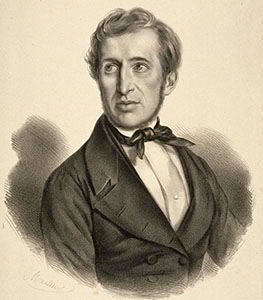
\includegraphics[height=\the\HauteurDesPhotos]{Mossotti}&
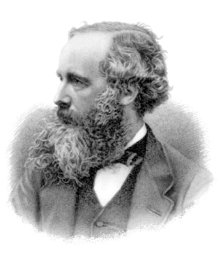
\includegraphics[height=\the\HauteurDesPhotos]{Maxwell}&
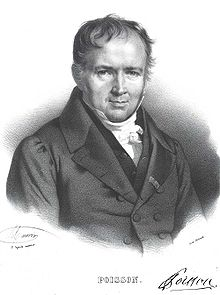
\includegraphics[height=\the\HauteurDesPhotos]{Poisson}&
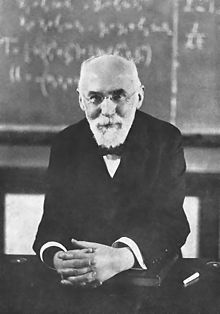
\includegraphics[height=\the\HauteurDesPhotos]{Lorentz}\\
Mossotti&Maxwell&Poisson&Lorentz%
\end{tabular}}

\medskip
\ImageADroite{%
Les premières théories remontent au \textsc{xix}\fup{e} siècle et sont dues à Mossotti,\index[aut]{Mossotti (Ottaviano-Fabrizio), 1791-1863, Italien} Maxwell,\index[aut]{Maxwell (James Clerk), 1831-1879, Écossais} Poisson\index[aut]{Poisson (Siméon Denis), 1781-1840, Français} ou encore Lorentz.\index[aut]{Lorentz (Hendrik Antoon), 1853-1928, Néerlandais} Le but de ces modèles est de fournir soit des bornes pour le comportement effectif, soit des approximations du comportement effectif. Les bornes sont optimales lorsqu'il existe une microstructure particulière qui réalise exactement le modèle physique. On évalue les «bonnes» propriétés de ces théories en les confrontant à d'autres résultats théoriques, calculs analytiques et numériques...}

\medskip
Ces théories sont utilisées pour les problèmes de conductivité (milieux diélectriques), en mécanique, magnétique, thermique... lorsque l'on a des phases de conductivité, d'élasticité, des coefficients thermiques... variables. Ces problèmes sont en général très difficiles à résoudre (non-linéaires et anisotropes) alors qu'en même temps, du point de vue des applications pratiques, il n'est pas forcément nécessaire de tenir compte de l'ensemble des degrés de liberté de ces systèmes.

\medskip
L'existence d'un \emph{comportement effectif}\index{effectif} n'est nullement assurée. On montre que, sous certaines hypothèses (en particulier l'existence d'un \emph{volume élémentaire représentatif}),\index{volume élémentaire représentatif} on peut effectivement remplacer un matériau hétérogène par un milieu homogène équivalent.

Enfin, d'un point de vue purement numérique, ces méthodes peuvent être utilisées pour «simplifier» un système à résoudre, que cela ait un sens physique ou non.
\end{histoire}

\medskip\colorgreen
Notons que les techniques d'homogénéisation ne sont pas que des artefacts, des trucs et astuces.
Certaines des grandeurs physiques que nous utilisons tous les jours ne sont que des moyennes. Le meilleur exemple en est la pression. Bien qu'en un point donné d'un gaz on voit passer des particules allant en tous sens, on constate également, à une échelle plus macroscopique, un schéma d'ensemble qui permet de définir par exemple la pression qu'exerce ledit gaz sur une paroi... pourtant rien de «cohérent» ne se dégage à l'échelle microscopique.\colorblack

\medskip
Le but de ce chapitre est donc d'effectuer le passage du niveau microscopique au niveau macroscopique (historiquement les premières homogénéisations, appelées alors moyennisations, utilisaient les moyennes arithmétique et harmonique) en fournissant la justification de ce passage (existence et unicité) ainsi que la formule (l'algorithme) de calcul des coefficients efficaces.

\medskip
Les méthodes que nous présenterons seront les \textcolorblue{méthodes de développement régulier, de la couche limite, et de développement asymptotique.} Le cas des \textcolorblue{milieux poreux} sera ensuite considéré. Enfin, nous mentionnerons une application de ces méthodes pour \textcolorblue{réduire la dimension} de certains problèmes.

\medskip
Une dernière remarque avant d'enter dans le vif du sujet, car elle correspond à des interrogations de nombreux étudiants: \textcolorred{il n'est pas nécessaire qu'un problème soit périodique pour pouvoir recourir aux techniques d'homogénéisation.} En effet, l'homogénéisation consiste à remplacer un problème «compliqué» par un «plus simple» selon une certaine «mesure»: il s'agit donc généralement de montrer que l'intégrale d'un truc compliqué peut s'écrire comme une autre intégrale d'un truc plus simple... et c'est l'égalité de ces deux intégrales qui fait que l'on dit que les problèmes sont équivalents (conduisent à la même solution), et donc que le second problème correspond à l'homogénéisation du premier. Dans le même ordre d'idée, et pour enfoncer le clou, \textcolorred{un matériau homogénéisé n'est par forcément isotrope.} En effet, on peut remplacer un matériau fortement anisotrope par un matériau homogénéisé isotrope, mais cela n'est pas forcément le plus adapté: il peut être préférable de l'homogénéiser en un matériau lui-même anisotrope mais «plus simple». Un matériau composite composé de plusieurs plis ayant des orientations différentes pourrait être remplacé par exemple par un matériau composite homogénéisé n'ayant qu'une couche (donc plus simple), mais restant anisotrope (qui serait, en quelque sorte, orienté selon une direction «homogénéisée», et il est alors plus «facile» de raisonner avec cette orientation «principale» lorsque l'on souhaite physiquement comprendre le comportement du matériau).


\medskip
\section{Méthodes d'homogénéisation}\index{homogénéisation}

Nous allons considérer le problème de conductivité linéaire donné par l'équation de Poisson\index[aut]{Poisson (Siméon Denis), 1781-1840, Français}\index{ED-EDP!de Poisson} avec condition de Dirichlet.\index[aut]{Dirichlet (Johann Peter Gustav Lejeune), 1805-1859, Allemand}\index{condition aux limites!de Dirichlet} Nous rappelons qu'il s'agit du problème suivant (qui décrit le déplacement vertical~$u$ d'une membrane plane):
\begin{equation}
\left\{
\begin{aligned}
&\dive(A(x)\nabla u) = f(x)&&\text{ pour } x\in\Omega\\
&u=0 &&\text{ sur } \Gamma=\partial\Omega
\end{aligned}
\right.
\end{equation}
On rappelle également que si~$\Omega$ est un ouvert connexe borné de~$\RR^n$, et $H_0^1(\Omega)$ l'espace de Sobolev des fonctions qui s'annulent sur~$\Gamma$, alors la solution $u\in H_0^1(\Omega)$ du problème précédent est également la solution du problème faible:
\begin{equation}
\forall v\in H_0^1(\Omega),\quad -\dint_\Omega A(x)\nabla u\cdot\nabla v = \dint_\Omega f(x)v
\end{equation}
où~$f\in L^2(\Omega)$.
Pour que ces deux formulation soient équivalentes, on a supposé que~$A(x)$ est régulière: i.e. que pour chaque~$x$ de~$\Omega$, $A(x)$ est une matrice~$n\times n$, dont les éléments sont mesurables et qui est symétrique, définie-positive, bornée, i.e. qu'il existe deux constantes~$K_1$ et~$K_2$~$>0$ telles que:
\begin{equation}\forall v\in\RR^n,\quad K_1 v\cdot v \le A(x) v\cdot v \le K_2 v\cdot v\end{equation}
Mentionnons le cas particulier où~$A(x)$ est régulier dans~$\Omega$ mais pas sur~$\Gamma$, alors on a deux conditions d'interface:
\begin{equation}
[u]=0 \quad\text{ et }\quad [n\cdot A(x)\nabla u]=0
\end{equation}
Nous savons également que la solution existe et est unique (d'après le théorème de Lax-Milgram,\index[aut]{Lax (Peter), 1926-, Américain}\index{théorème!de Lax-Milgram}\index[aut]{Milgram (Arthur Norton), 1912-1961, Américain} i.e. d'après le théorème de Riesz-Fréchet\index[aut]{Riesz (Frigyes), 1880-1956, Hongrois}\index{théorème!de représentation de Riesz-Fréchet}\index[aut]{Fréchet (Maurice René), 1878-1973, Français} en remarquant le produit scalaire qui va bien...)

\medskip
Intéressons nous maintenant d'un peu plus près à~$A(x)$.
Supposons que~$A(x)$ possède une certaine périodicité~$\varepsilon$, par exemple, que le matériau constituant le domaine soit constitué de couches successives de deux matériaux différents, mais avec une périodicité, comme illustré sur la~\fig{Fig-Ax}.
\begin{figure}[ht]
\centering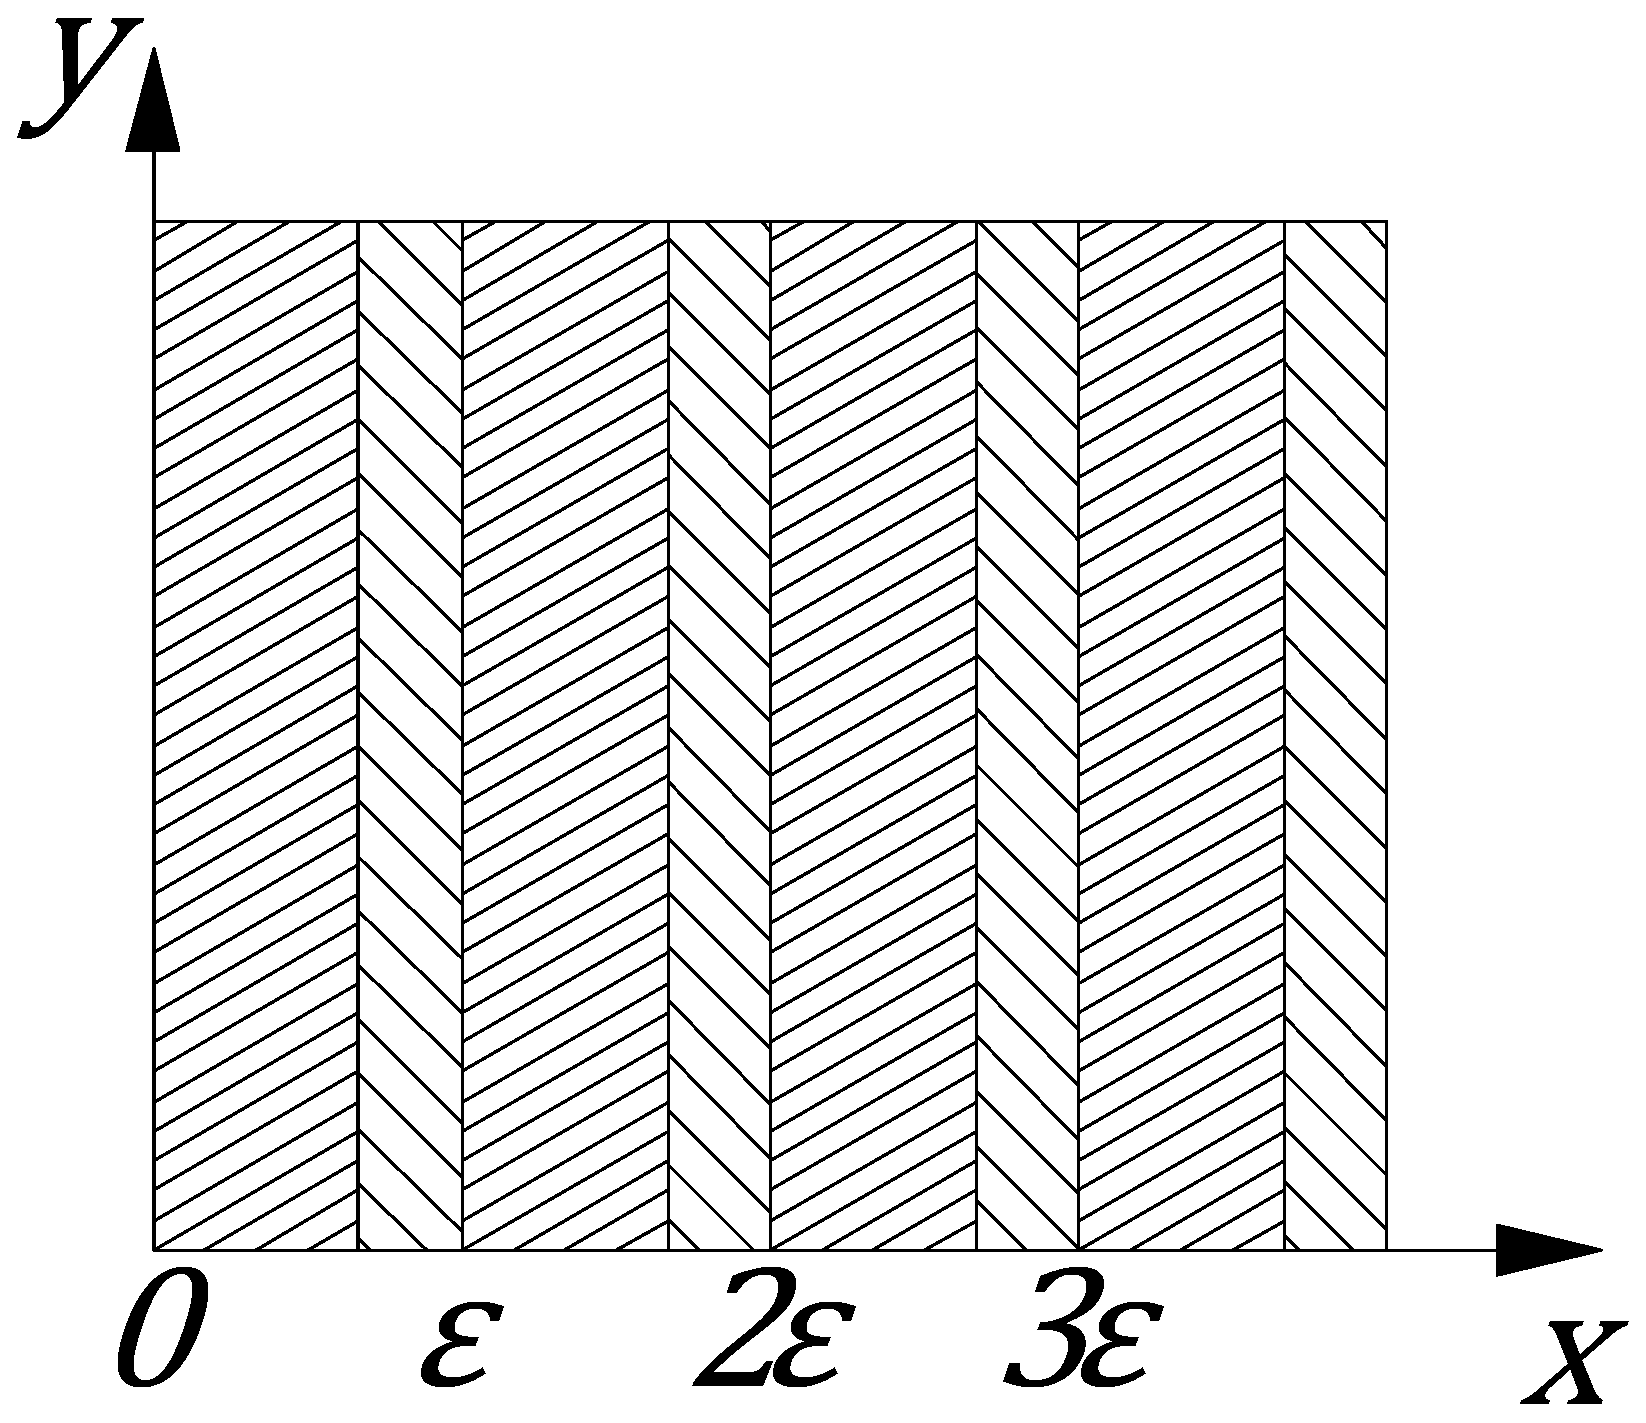
\includegraphics[height=35mm]{Ax.eps}
\caption{Matériau périodique}\label{Fig-Ax}
\end{figure}
Dans un tel cas, nous dirons que les coefficients~$A$ dépendent de~$x/\varepsilon$. Cette écriture sous forme normalisée permet de dire que~$A$ est périodique de période 1.

\medskip
Dans le cas unidimensionnel, le problème devient:
\begin{equation}
\left\{
\begin{aligned}
&\dfrac \dd{\dd x}\left(A\left(\frac x\varepsilon\right)\right) \dfrac{\dd u}{\dd x} = f(x)&& \text{ pour } x\in[0,l]\\
&u=0 &&\text{ pour } x=0 \text{ et } x=l
\end{aligned}
\right.
\end{equation}
$A$ est une fonction de~$\RR$ dans~$\RR$ de période 1, et nous la supposerons régulière par morceaux et telle qu'il existe~$K_1$ et~$K_2$~$>0$ telles que~$K_1\le A(v)\le K_2$.

\medskip
La solution du problème est alors:
\begin{equation}
u(x)=\dint_0^x A^{-1}(y/\varepsilon) \left(\dint_0^y f(v)\dd v + c_1 \right) \dd y + c_2
\end{equation}
avec~$c_2=0$ et
\begin{equation} c_1 = \dfrac{\dint_0^l A^{-1}(y/\varepsilon)\dint_0^y f(v)\dd v \dd y}{\dint_0^l a^{-1}(y/\varepsilon)\dd y} \end{equation}
Le nombre d'intervalles pour le calcul approché de~$c_1$ est très grand (i.e. très supérieur à~$l/\varepsilon$).

Exprimé autrement, ce résultat devient: \textcolorblue{le coefficient homogénéisé est~$1/\langle\frac1A\rangle$} et non pas~$\langle A\rangle$ (où~$\langle\cdot\rangle$ désigne la moyenne).


\medskip
\subsection{Méthode de développement régulier}\index{méthode de développement régulier}

Dans la \textcolorblue{méthode de développement régulier}, on se propose de chercher la solution asymptotique~$u^{(\infty)}$ sous la forme:\index{méthode de développement régulier}
\begin{equation}
u^{(\infty)} \sim \dsum_{i=0}^\infty \varepsilon^iu_i(x)
\end{equation}
\textcolorred{où~$u_i(x)$ ne dépend pas de~$\varepsilon$.}

\medskip
La solution asymptotique~$u^{(\infty)}$ est bien de la forme précédente si en injectant cette expression dans celle du problème alors on obtient une petite erreur au second membre.

\medskip
Pour le calcul on procède donc comme suit:
\begin{itemize}
  \item on injecte la forme souhaitée (cette forme s'appelle \textcolorblue{l'ansatz});\index{ansatz}
  \item pour avoir un second membre avec un terme d'erreur petit, on obtient la forme des~$u_i(x)$;
  \item on vérifie que les~$u_i(x)$ trouvés conviennent bien.
\end{itemize}


\medskip
\subsection{Méthode de la couche limite}\index{méthode de la couche limite}

Considérons le problème unidimensionnel:
\begin{equation}
\left\{
\begin{aligned}
&\varepsilon^2u''-p(x)u= f(x) &&\text{ pour } x\in\intff{0}{1}\\
&u(0)=A \text{ et } u(1)=B
\end{aligned}
\right.
\end{equation}
où~$p\in C(\intff{0}{1})$;~$p(x)\ge0, x\in\intff{0}{1}$;~$f\in C(\intff{0}{1})$;~$A\in\RR$, $B\in\RR$ et
$\varepsilon>0$ le petit paramètre.
En négligeant le terme~$\varepsilon^2 u''$, nous arrivons à l'équation~$-p(x)u_r=f(x)$.
\begin{figure}[ht]
\centering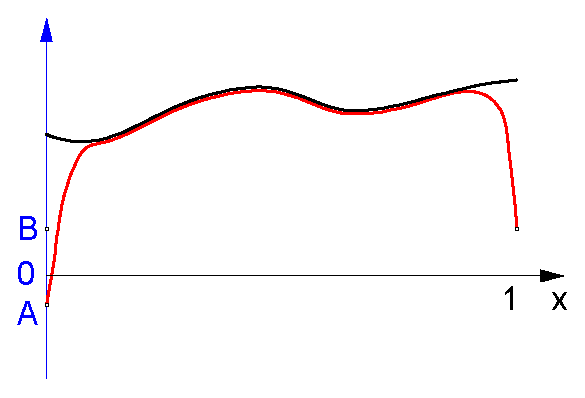
\includegraphics[height=50mm]{clim.eps}
\caption{Méthode de la couche limite}\label{Fig-clim}
\end{figure}
En d'autres termes, et comme montré sur la \fig{Fig-clim}, nous disposons de la courbe correspondant à~$y=u_r=-f(x)/p(x)$ (en noir) qui approche la solution du problème donnée par la courbe rouge.
%La courbe noire correspond à~$y=u_r=-f(x)/p(x)$, et la courbe rouge à la solution du problème.

La solution exacte se confond avec~$u_r$ sur la plus grande partie de l'intervalle~$\intff{0}{1}$,
mais~$u$ et~$u_r$ sont fortement différents dans un voisinage des extrémités.

\medskip
Cherchons une solution asymptotique sous la forme de l'ansatz:\index{ansatz}
\begin{equation}
u^{(\infty)} \sim \dsum_{i=0}^\infty \varepsilon^i\left( u_i^r(x) + u_i^0(x/\varepsilon)
+u_i^1((x-1)/\varepsilon) \right)
\end{equation}
où les~$u_i^r(x)$ sont les \textcolorblue{termes réguliers}, et~$u_i^0(x/\varepsilon)$ et
$u_i^1((x-1)/\varepsilon)$ les \textcolorblue{termes de couche limite} correspondant aux
extrémités~$x=0$ et~$x=l$.

\medskip
Pour le calcul on procède donc comme suit:
\begin{itemize}
  \item on injecte les termes réguliers de l'ansatz\index{ansatz} dans la formulation du problème;
  \item on traite les extrémités pour vérifier les conditions aux limites, ce qui donne les termes de couche
	limite;
  \item on vérifie que la solution trouvés conviennent bien (i.e. que l'erreur commise est négligeable).
\end{itemize}


\medskip
\subsection{Méthode de développement asymptotique infini}\index{méthode de développement asymptotique infini}

À ce niveau du texte, on a dû s'apercevoir que la démarche était la même pour les deux méthodes précédentes, sauf évidemment la forme de l'ansatz.\index{ansatz}
Dans la \textcolorblue{méthode de développement asymptotique infini}, on va encore procéder de la même manière, mais on cherchera une solution sous la forme d'ansatz:\index{ansatz}
\begin{equation}
u^{(\infty)} \sim \dsum_{i=0}^\infty \varepsilon^i u_i(x,x/\varepsilon)
\end{equation}
où chaque~$u_i(x,x/\varepsilon)$ est de la forme~$u_i(x,x/\varepsilon)=N_i(x/\varepsilon)v_\varepsilon^{(i)}(x),
\forall i>0$ et~$u_0(x,x/\varepsilon)=v_\varepsilon(x)$, i.e.:
\begin{equation}
u^{(\infty)} \sim \dsum_{i=0}^\infty \varepsilon^i N_i(x/\varepsilon)v_\varepsilon^{(i)}(x)
\end{equation}
et où les~$N_i(x/\varepsilon)$ sont 1-périodiques et~$N_0=1$.

\medskip
\textcolorgris{Pour un détail plus mathématique, on pourra se référer par exemple à~\cite{bib-Allaire2scale} qui présente la notion de convergence à deux échelles («Two-scale convergence»). Cet article, bien qu'un peu technique, reste relativement abordable.}

\medskip
\subsection{Cas des coefficients discontinus}

Il est possible d'appliquer la même approche que lorsque les coefficients sont continus avec quelques modifications: il «suffit» d'ajouter les conditions d'interfaces présentées en début de paragraphe et rappelées ci-dessous:
\begin{equation} [u]=0 \quad \text{ et } \quad [n\cdot A(x/\varepsilon)\nabla u] = 0\end{equation}
partout où cela est nécessaire.

On retrouve les mêmes conditions d'existence de la solution que dans le cas continu et la périodicité de la solution homogénéisée reste inchangée.



\medskip
\section{Homogénéisation simplifiée pour les matériaux composites}\index{homogénéisation}

Après ce petit tour «mathématique» des méthodes d'homogénéisation, nous proposons un petit complément très mécanique, et très «pratique».

\medskip
Pour information, la modélisation du muscle cardiaque s'inspire des techniques d'homogénéisation des matériaux composites.


\medskip
\subsection{Introduction}

D'une manière générale, tous les matériaux, mêmes isotropes, sont hétérogènes en dessous d'une certaine échelle. Il peut sembler naturel d'utiliser des propriétés homogènes équivalentes correspondant à des propriétés mécaniques effectives. Toutefois, comme nous l'avons déjà vu, ces propriétés effectives\index{effectif} ne s'obtiennent pas par une simple moyenne des propriétés des constituants, mêmes pondérées par les fractions volumiques.

\medskip
Les propriétés effectives du milieu homogène équivalent cherché peuvent être obtenues en résolvant un problème aux limites sur un \textcolorblue{volume élémentaire}~$dV$, à condition que celui-ci soit \textcolorblue{suffisamment grand pour être représentatif de la microstructure du matériau hétérogène.}\index{volume élémentaire représentatif} Dans le cas où les constituants présentent une structure périodique, le volume~$dV$ peut se réduire à un \textcolorblue{volume élémentaire}.

\medskip
Une fois le volume élémentaire déterminé, on le soumet à des sollicitations élémentaires pour déterminer la réponse résultante. \textcolorred{La difficulté réside en fait dans le choix des conditions aux limites à appliquer au volume élémentaire considéré pour imposer une déformation ou contrainte globale moyenne donnée.}
Dans le cas linéaire, on peut prouver l'existence et l'unicité pour les différents cas de conditions aux limites existants.

\medskip
Principalement pour les composites stratifiés ou sandwichs, il y a deux niveaux d'homogénéisation:
\begin{itemize}
	\item du niveau micromécanique au niveau mésoscopique:
		Les hétérogénéités de base sont les fibres et la matrice. On effectue ici
		 une étape d'homogénéisation locale.
	\item du niveau mésoscopique au niveau macroscopique:
		Les hétérogénéités de base sont les différentes couches du stratifié.
		 Ces couches sont considérées comme «homogènes» (étape précédente).
		 Cette fois, il s'agit d'une homogénéisation dans l'épaisseur du stratifié.
\end{itemize}

\medskip
On pourra par exemple se reporter à~\cite{bib-Corrugated} pour voir comment cela est utilisé pour développer un modèle de plaque homogénéisée équivalente à un matériau fait de carton ondulé entre deux peaux de carton.

\medskip
\subsection{Loi des mélanges, bornes de Voigt et de Reuss}\index{loi!des mélanges}\index{borne!de Voigt}\index{borne!de Reuss}\index[aut]{Voigt (Woldemar), 1850-1919, Allemand}

On considère un composite UD (unidirectionnel) de repère d'orthotropie~$(l,t)$, constitué de fibres noyées dans une matrice polymère. Soit une cellule élémentaire de fraction volumique~$V = 1$ constituée de fibres et de matrice. On note $V_m$ la fraction volumique de matrice, $V_f$ la fraction volumique de fibre, et on a:
\begin{equation} V = V_m + V_f =1 \end{equation}
\medskipvm
À l'échelle locale, on fait les hypothèses suivantes:
\begin{itemize}
  \item Fibres: comportement élastique linéaire fragile isotrope de coefficients~$E_f$ et~$\nu_f$;
  \item Matrice: comportement élastique non-linéaire, isotrope de coefficients~$E_m$ et~$\nu_m$.
\end{itemize}
\medskipvm
On souhaite déterminer les relations existant entre~$E_l$, $E_t$, $E_f$, $E_m$, $V_m$ et~$V_f$.
\medskipvm
Pour cela, on fait également les hypothèses suivantes:
\begin{itemize}
  \item On travaille en élasticité linéaire.
  \item La liaison fibres/matrice est parfaite.
  \item Localement, on a:~$\sigma_f = E_f \varepsilon_f$ et~$\sigma_m = E_m \varepsilon_m$.
\end{itemize}
\medskipvm
Loi des mélanges (ou modèles à bornes ou de Reuss et de Voigt):
\begin{itemize}
	\item premier essai --- Il s'effectue dans la direction parallèle aux fibres (compression longitudinale)
		\begin{equation} E_{\text{longitudinal}}=E_l=E_fV_f+E_mV_m \end{equation}
		C'est la loi des mélanges, qui est bien vérifiée dans la direction des fibres.
		Il s'agit de la borne supérieure de Voigt (1887).\index{loi!des mélanges}\index{borne!de Voigt}\index[aut]{Voigt (Woldemar), 1850-1919, Allemand}
	\item deuxième essai --- Il s'effectue dans la direction perpendiculaire aux fibres (compression transversale)
		\begin{equation}\dfrac1{E_{\text{transverse}}}=\dfrac1{E_t} = \dfrac{V_f}{E_f}+\dfrac{V_m}{E_m}\end{equation}
		C'est la loi des mélanges en souplesse.
		Cette relation n'est pas très bien vérifiée transversalement mais donne une
		indication sur la borne inférieure, dite de Reuss (1929).\index{loi!des mélanges}\index{borne!de Reuss}
	\item Module de cisaillement et coefficient de Poisson\index[aut]{Poisson (Siméon Denis), 1781-1840, Français}
		\index{coefficients de Poisson}d'un UD par la loi des mélanges:\index{loi!des mélanges}
		\begin{equation}\nu_{lt}=\nu_fV_f+\nu_mV_m\quad\text{ et }\quad\dfrac1{G_{lt}} = \dfrac{V_f}{G_f}+\dfrac{V_m}{G_m}\end{equation}
\end{itemize}
%%%%%%%%%%%%%%%
\medskipvm
Les modèles à bornes fournissent un encadrement du comportement mécanique du matériau composite par des comportements mécaniques limites (bornes). Ils sont obtenus par la résolution du problème de l'élasticité linéaire sous forme faible. La minimisation de l'énergie potentielle conduit à la borne supérieure de Voigt.\index{borne!de Voigt}\index[aut]{Voigt (Woldemar), 1850-1919, Allemand} la résolution en contrainte conduit à la borne inférieure de Reuss.\index{borne!de Reuss}
\medskipvm
Pour gagner un peu en généralité, on peut remplacer les termes fibres et matrice par des phases, car ces modèles sont applicables à des mélanges de polymères (matériaux composés)
et à des composites chargés par des particules diverses. 

Les bornes correspondent aux associations série des deux phases (borne inférieure de Reuss,\index{borne!de Reuss} équivalent au modèle du module transverse équivalent de la loi des mélanges) et parallèle (borne supérieure de Voigt,\index{loi!des mélanges}\index{borne!de Voigt}\index[aut]{Voigt (Woldemar), 1850-1919, Allemand} équivalent au modèle du module longitudinal équivalent de la loi des mélanges).

Aucune hypothèse n'est faite sur la morphologie du matériau. Il est simplement admis que pour le modèle de Reuss, la contrainte est homogène dans les deux phases (continuité de la contrainte) et, pour le modèle de Voigt,\index[aut]{Voigt (Woldemar), 1850-1919, Allemand}
la déformation est constante (continuité de la déformation) dans tout le composite. \textcolorred{L'intérêt est limité dès que l'écart des caractéristiques des deux phases est important.}
\medskipvm
Évidemment, d'autres modèles existent:
\begin{itemize}
	\item Hashin et Shtrikman (1963): resserre les bornes de Reuss et Voigt
	\item Takayanagi (combinaison de Reuss et Voigt)
	\item Halpin - Tsaï: pour le renforcement par des fibres courtes alignées
	\item Tsaï - Pagano: fibres courtes
	\item Halpin - Kardos: extension de la précédente
\end{itemize}

\medskip
\section{Homogénéisation des matériaux poreux}

Considérons à nouveau notre problème de Poisson avec conditions de Dirichlet pour un milieu poreux.\index[aut]{Poisson (Siméon Denis), 1781-1840, Français}\index{ED-EDP!de Poisson}\index[aut]{Dirichlet (Johann Peter Gustav Lejeune), 1805-1859, Allemand}\index{condition aux limites!de Dirichlet} $\Omega$ est le domaine (borné) de~$\RR^n$ qui contient~$\Omega_\varepsilon$ l'ensemble des trous périodiques. Nous avons donc:
\begin{equation}
\left\{
\begin{aligned}
&\dive(A(x)\nabla u) = f(x) &&\text{ pour } x\in\Omega\backslash\Omega_\varepsilon\\
&u=0 && \text{ sur le contour extérieur } \Gamma=\partial\Omega\\
\end{aligned}
\right.
\end{equation}
Sur le bord des trous, on peut imposer, soit des conditions de Dirichlet:
\begin{equation}u=0 \end{equation}
soit des conditions de Neumann:\index[aut]{Neumann (Carl Gottfried), 1832-1925, Allemand}\index{condition aux limites!de Neumann}
\begin{equation}n\cdot A(x/\varepsilon)\nabla u=0 \end{equation}
On supposera encore que les coefficient sont 1-périodiques.

\medskip
\textcolorblue{Cherchons des solutions dans le cas où l'on a des conditions de Neumann sur le bords des trous.}\index[aut]{Neumann (Carl Gottfried), 1832-1925, Allemand}\index{condition aux limites!de Neumann}

La forme choisie pour l'ansatz\index{ansatz} est le développement au second ordre suivant:
\begin{equation}u^{(2)} = u_0(x,x/\varepsilon)+\varepsilon u_1(x,x/\varepsilon) + \varepsilon^2 u_2(x,x/\varepsilon)\end{equation}
où les~$u_i(x,x/\varepsilon)$ sont 1-périodiques en~$x/\varepsilon$ qui sera noté~$\xi$.

On obtient un système du type:
\begin{equation}\left\{
\begin{aligned}
&L_{\xi\xi} u_0 &&=0\\
&L_{\xi\xi}u_1+L_{\xi x}u_0+L_{x\xi}u_0 &&=0\\
&L_{\xi\xi}u_2+L_{\xi x}u_1+L_{x\xi}u_1 +L_{xx}u_0 &&=f(x)
\end{aligned}
\right. \end{equation}
et les conditions de Neumann:\index[aut]{Neumann (Carl Gottfried), 1832-1925, Allemand}\index{condition aux limites!de Neumann}
\begin{equation} n\cdot A(\xi)\left[ \varepsilon^{-1}\nabla_\xi u_0 + \varepsilon^0 (\nabla_\xi u_1+\nabla_x u_0) +
\varepsilon(\nabla_\xi u_2+\nabla_x u_1)+\varepsilon^2\nabla_x u_2
\right]=0 \end{equation}
d'où:
\begin{equation}\left\{
\begin{aligned}
&n\cdot A(\xi)\nabla_\xi u_0 &&=0\\
&n\cdot A(\xi) (\nabla_\xi u_1+\nabla_x u_0) &&=0\\
&n\cdot A(\xi)(\nabla_\xi u_2+\nabla_x u_1) &&=0
\end{aligned}
\right. \end{equation}
On peut prouver que si~$v_0$ est solution du problème, alors~$v_0+\text{cte}$ aussi.
\medskipvm
Des conditions d'existence de la solution il vient, tous calculs faits, la matrice des
coefficients homogénéisés~$\hat{A}$:
\begin{equation} \hat{A} = [\hat{a}_{i,j} ]
\quad \text{ avec }
\quad
\hat{a}_{i,j}=\dint_{Q\backslash G_0} \dsum_{k=1}^n \left(a_{ik} \frac{\partial N_j}{\partial\xi_k} + a_{ij}
\right) \dd\xi
\end{equation}
où~$G_0$ est un trou de la cellule élémentaire~$Q$.
\medskipvm
Le même type de calcul pourrait être mené avec les conditions de Dirichlet sur le bord des trous.
\medskipvm
Cette homogénéisation des milieux poreux est valable pour l'acoustique comme pour la mécanique.

\medskip
\section{Homogénéisation des problèmes non stationnaires}

Nous n'avons pas encore abordé de manière pratique les problèmes non stationnaires dans ce document, puisqu'ils se trouvent au chapitre~\ref{Ch-temps}.

Il est tout à fait possible d'utiliser les méthodes présentées dans ce chapitre aux problèmes dépendant du temps. Il n'y a pas vraiment de précautions supplémentaires à prendre, mais il faut adapter la forme de l'ansatz.\index{ansatz} Par exemple, l'ansatz\index{ansatz} du paragraphe précédent, pour le même type de problème non stationnaire serait:
\begin{equation}u^{(2)} = u_0(x,\xi,t)+\varepsilon u_1(x,\xi,t) + \varepsilon^2 u_2(x,\xi,t)\end{equation}
avec~$u_i(x,\xi,t)$ 1-périodique en~$\xi$.

\medskip
\section{Changement de dimension et raccord de maillage}

\textcolorgreen{Les méthodes d'homogénéisation peuvent également être utilisées pour «changer (réduire)» la dimension d'un problème.}

\medskip
Considérons un problème qui se pose dans un domaine plan de longueur~$1$ et de largeur~$\pm\varepsilon/2$. Alors, on peut considérer le comportement asymptotique de la solution lorsque~$\varepsilon \longrightarrow 0$. Une fois cette solution asymptotique trouvée, le problème initial posé sur le pavé $\intff{0}{1}\times[-\varepsilon/2,+\varepsilon/2]$ est remplacé par le problème homogénéisé posé sur le segment~$\intff{0}{1}$. On a donc bien réduit la dimension du problème.

\medskip
Ce genre de chose correspond typiquement à un modèle plaque ou coque (2D) utilisé à la place d'un modèle tridimensionnel (3D), ou encore mieux à un modèle barre ou poutre (1D).

Cela permet également de développer des éléments finis permettant de raccorder des maillages 3D à des maillages 2D ou à des maillages 1D, afin d'alléger les modèles numériques là où ils peuvent l'être.

\medskip
En mécanique, de nombreuses théories de plaques ou poutres existent (voir la paragraphe~\ref{Sec-PlusModel}). Elles sont généralement présentées de manières «physique», mais ne sont rien d'autre que des méthodes d'homogénéisation.

Libre à chacun de préférer une présentation plutôt mécanicienne ou plutôt mathématicienne, le résultat est finalement le même. Mais il nous semble, et c'est la motivation même à l'origine de ce document, que le fait de connaître les deux aide à mieux cerner à la fois les \textcolorblue{hypothèses} sur lesquelles ces développements sont faits (et que l'on oublie parfois, ayant pour conséquence des résultats que l'on peut qualifier de surprenants) ainsi que les \textcolorblue{potentialités} qui s'offrent à nous. 
